\chapter{Flight Data \label{ch:flight_data}}
After having found the set of optimal calibration parameters and applying them to the flight data of \ac{SETH} junior, roll and pitch angles as well as the gondolas heading or orientation can be calculated. How this is done has been described in sec. \ref{sec:meth:determination_heading} on page \pageref{sec:meth:determination_heading}.

The upper plot in fig. \ref{fig:res:flight_heading} presents the pitch angle in red and roll angle in blue plotted against the time. The lower plot presents the gondolas heading against time. The angle of heading is given from 0$^\circ$ to 360$^\circ$ as it is written on a compass with $0^\circ\equiv\mathrm{North}$, $90^\circ\equiv\mathrm{East}$, etc.\\
It can be seen that the gondola's swinging is strongest after launch and during ascent until it calms down at higher altitudes.\\
The timestamp on the x-axis has been corrected to show the correct time in~UTC. The Raspberry~Pi has an internal clock which is used during flight. If the time is not set it continues counting up from the time when it was last shut off. This resulted in a time difference of 3443\,s that the Pi was behind.

\begin{figure}[H]
    \centering
    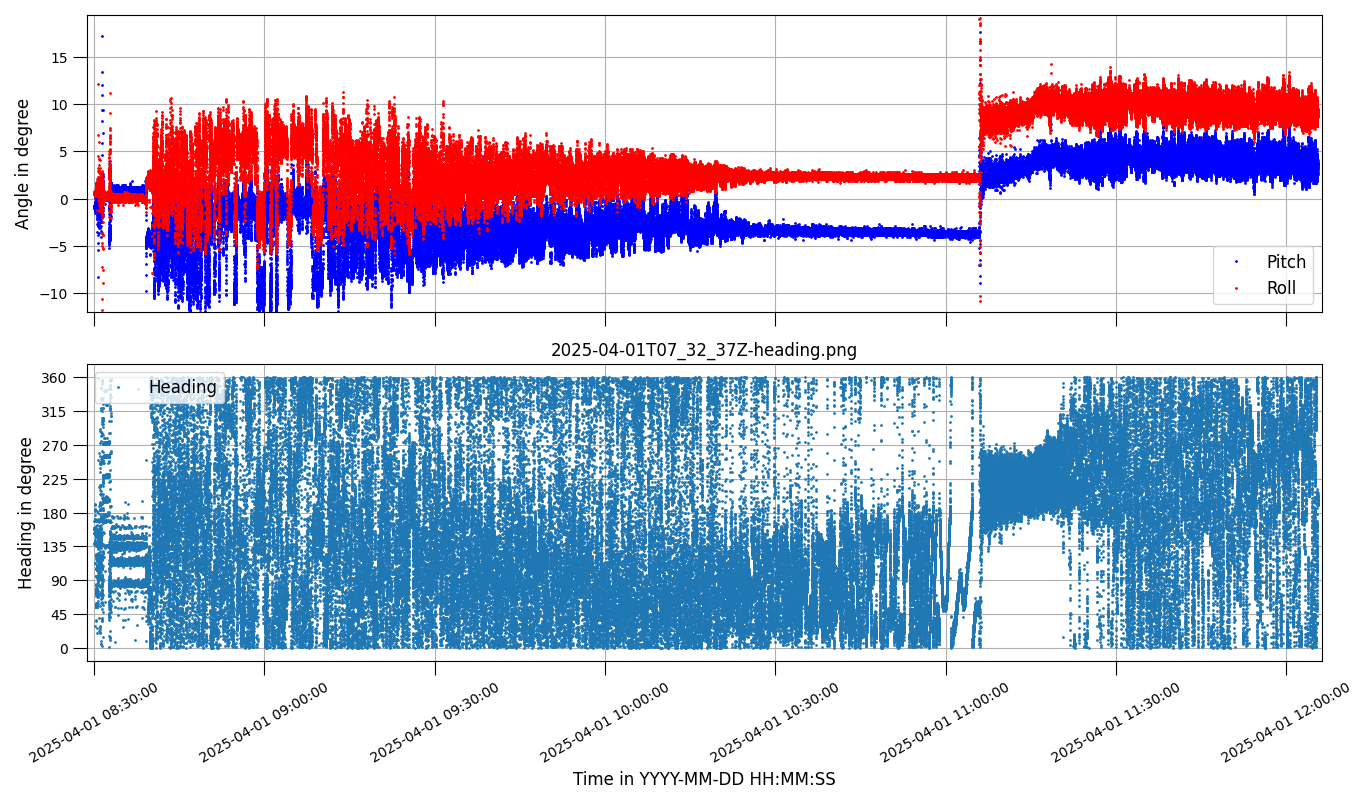
\includegraphics[width=\linewidth]{images/04_results/flight_heading.png}
    \caption{Pitch, roll and heading during the whole flight.}
    \label{fig:res:flight_heading}
\end{figure}

Launch of the balloon was around 10:40 local time or 8:40~UTC. After this time the balloon started its ascent, the gondola swinging and rotating below it. The swinging gradually decreases with time and altitude until it is calmest before the burst. The rotational frequency is seemingly constant but also decreases before the burst of the balloon. After balloon burst the payload rocks around the South-South-West direction and continues swinging. As the red curve is shifted upwards it can be assumed that the parachute does not decelerate the gondola uniformly but pulls it to one side.

\section{Launch \label{sec:launch}}
The balloon was launched just before 10:40~LT, 8:40~UTC as shown below in fig. \ref{fig:res:launch_heading}. The Figure is held in the same style as described in the previous section. In the lower plot presenting the heading, it can be seen that there is a time interval between 8:33 until launch where the heading is not stable at one single value the three bands lie at respectively. I cannot explain this as the magnetometer measurement for the still and moved magnetometer dont show this structure in \ref{fig:res:raw_cali_vectors} (page \pageref{fig:res:raw_cali_vectors}).\\
It can be seen that the gondola rotates quickly at about 5 revolutions per minute (rpm). Swinging of the gondola is also strong with a peak-to-peak amplitude of around 10$^\circ$ in roll and pitch. In the first ten minutes the roll angle is relatively symmetrical around 0 while the pitch angle is centred around the -5$^\circ$ mark. This can be explained by the balloon pulling the gondola with it in the wind direction.

\begin{figure}[H]
    \centering
    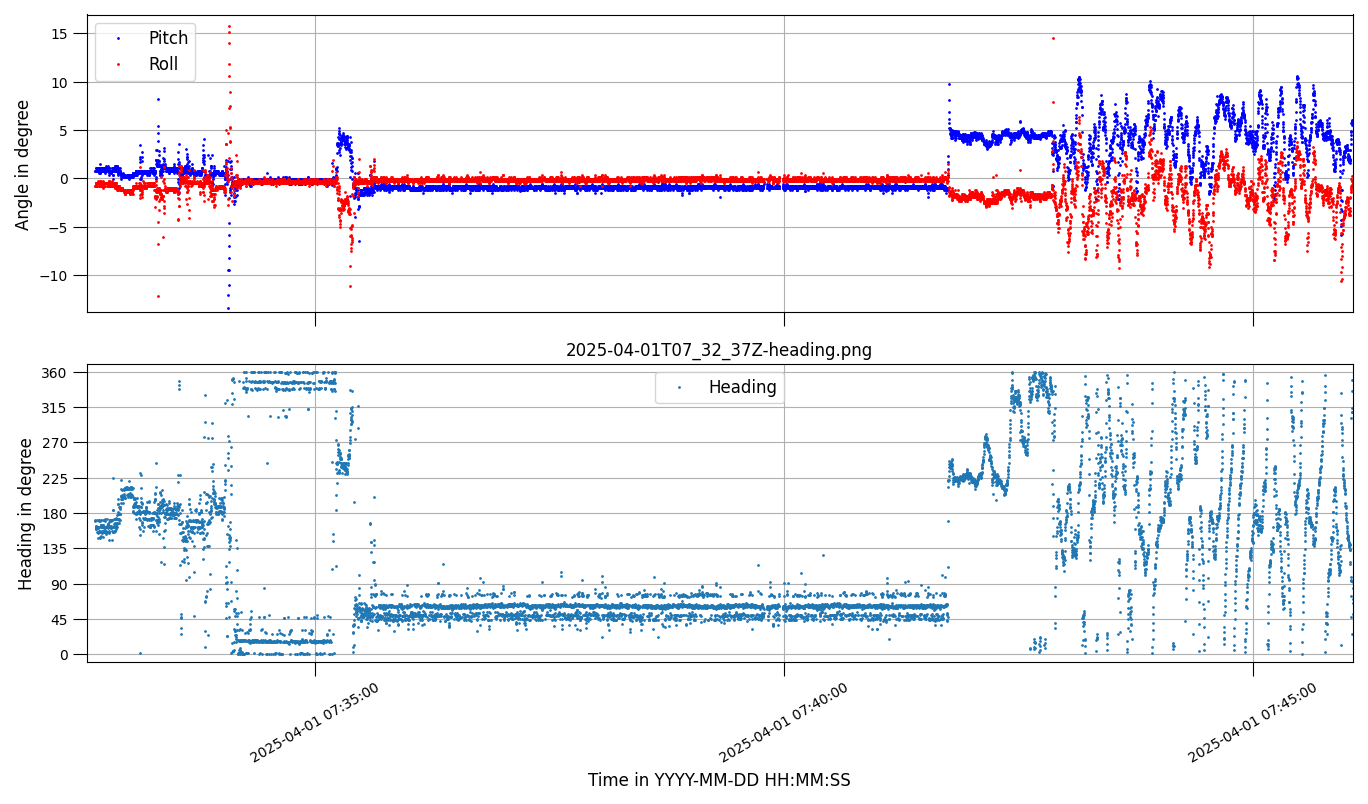
\includegraphics[width=\linewidth]{images/04_results/launch_heading.png}
    \caption[Heading at launch.]{Pitch, roll and heading around launch.}
    \label{fig:res:launch_heading}
\end{figure}


\section{Ascent \label{sec:ascent}}
In Figure \ref{fig:res:ascent_heading} it can be seen that the rotation of the gondola has slowed down to approximately 4~rpm. The swinging went down significantly to a peak-to-peak amplitude of 2 to 5 degrees. The wind direction seems to have turned by 90 degrees as now the roll is offset by 10 degrees rather than the pitch. Some periods (e.g. 9:04 - 9:05) again show a different wind direction than the rest of the time.

\begin{figure}[H]
    \centering
    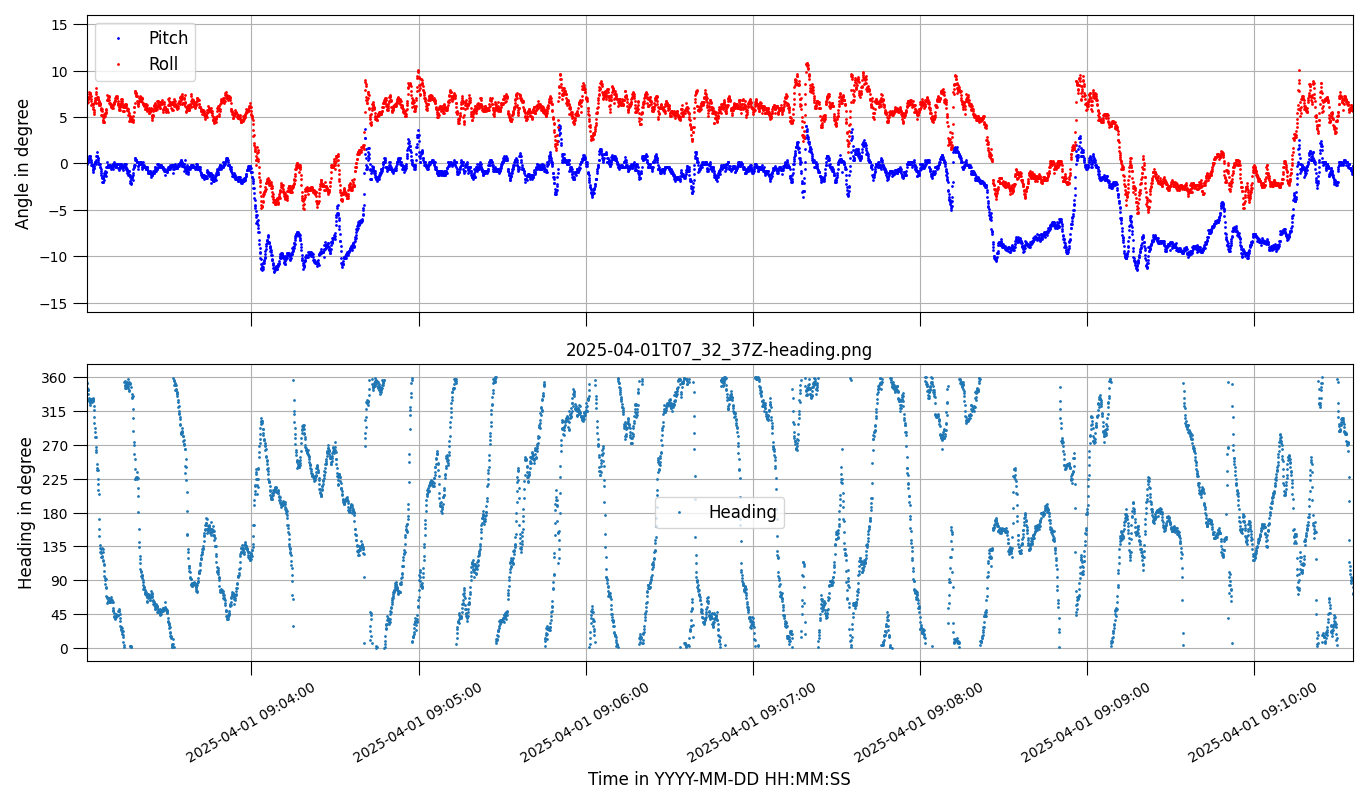
\includegraphics[width=\linewidth]{images/04_results/mid_flight_heading.png}
    \caption[Heading during ascent.]{Pitch, roll and heading during ascent.}
    \label{fig:res:ascent_heading}
\end{figure}


\section{Balloon Burst \label{sec:balloon_burst}}
The balloon burst at approx. 11:06~UTC as can be seen in fig.\ref{fig:res:burst_heading}. It can also be seen in the upper plot that the roll and pitch angles are constantly different from zero. In addition to the movement of the gondola being dragged behind the balloon, may be the weight distribution of the payload. Until now it was assumed that the floor of the polystyrene box hanging from the balloon would be parallel to the ground when hung from its cover. If the attachment of the rope is not exactly in the middle of the cover but off in any direction, the box might hang a little bit inclined. This has not been tested for as the gondola only ever sat on the ground. 

\begin{figure}[H]
    \centering
    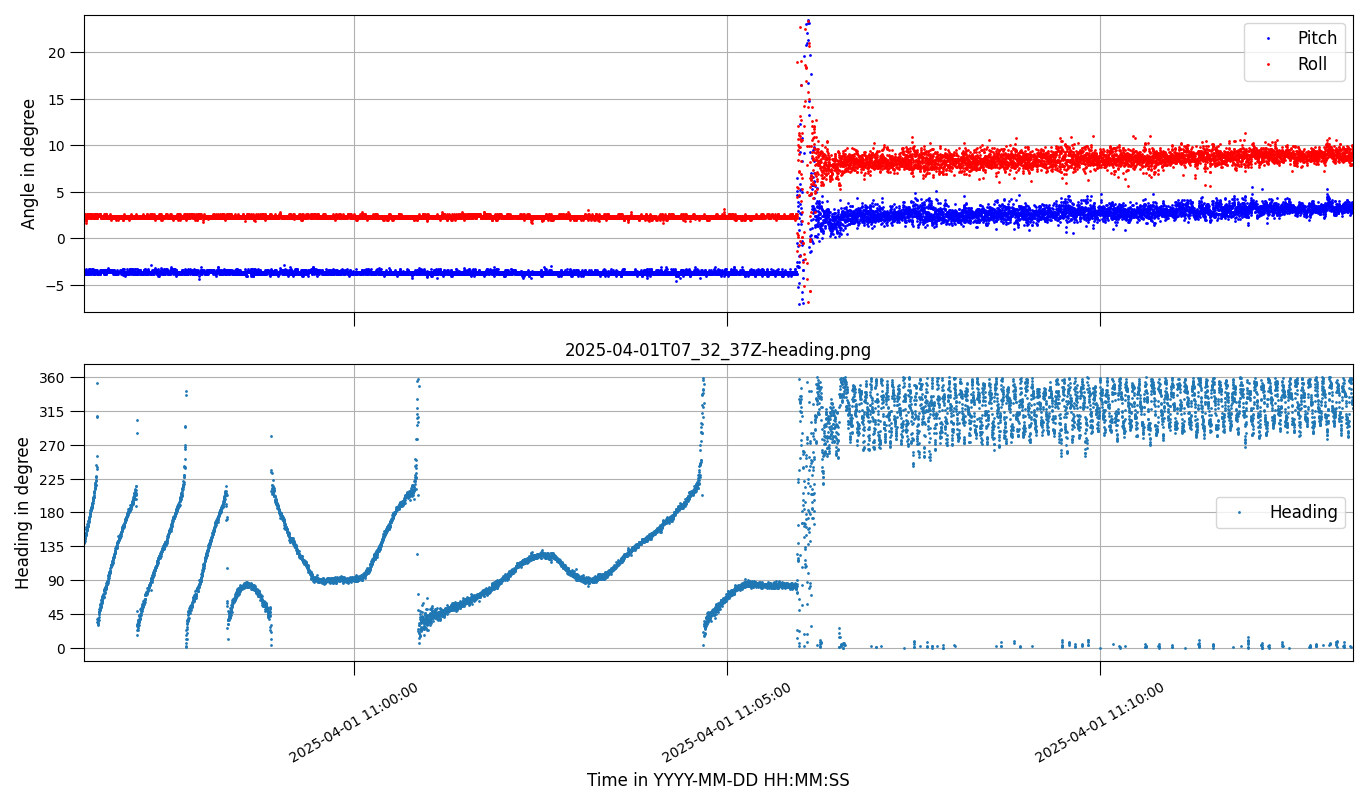
\includegraphics[width=\linewidth]{images/04_results/pop_heading.png}
    \caption[Heading at balloon burst.]{Pitch, roll and heading balloon burst.}
    \label{fig:res:burst_heading}
\end{figure}


\section{Descent \label{sec:descent}}
The last flight phase is the descent of the payload. At this time a parachute has opened and is producing drag to slow the box to an equilibrium velocity. As can be seen in fig. \ref{fig:res:descent_heading}, roll and pitch angle are offset by 5 and 10 degrees each. This may be again because the attachment of the parachute is not perfectly centred and the centre of gravity is not in the centre of the box. Each has a peak-to-peak amplitude of approx. $5^\circ$.\\
In the lower plot in fig. \ref{fig:res:descent_heading} it can be seen that the gondola is not spinning after the burst. Sporadically the box will perform a rotation which gets more frequent until about 11:32~UTC when the gondola begins to spin with a frequency of approx. 5~rpm.

\begin{figure}[H]
    \centering
    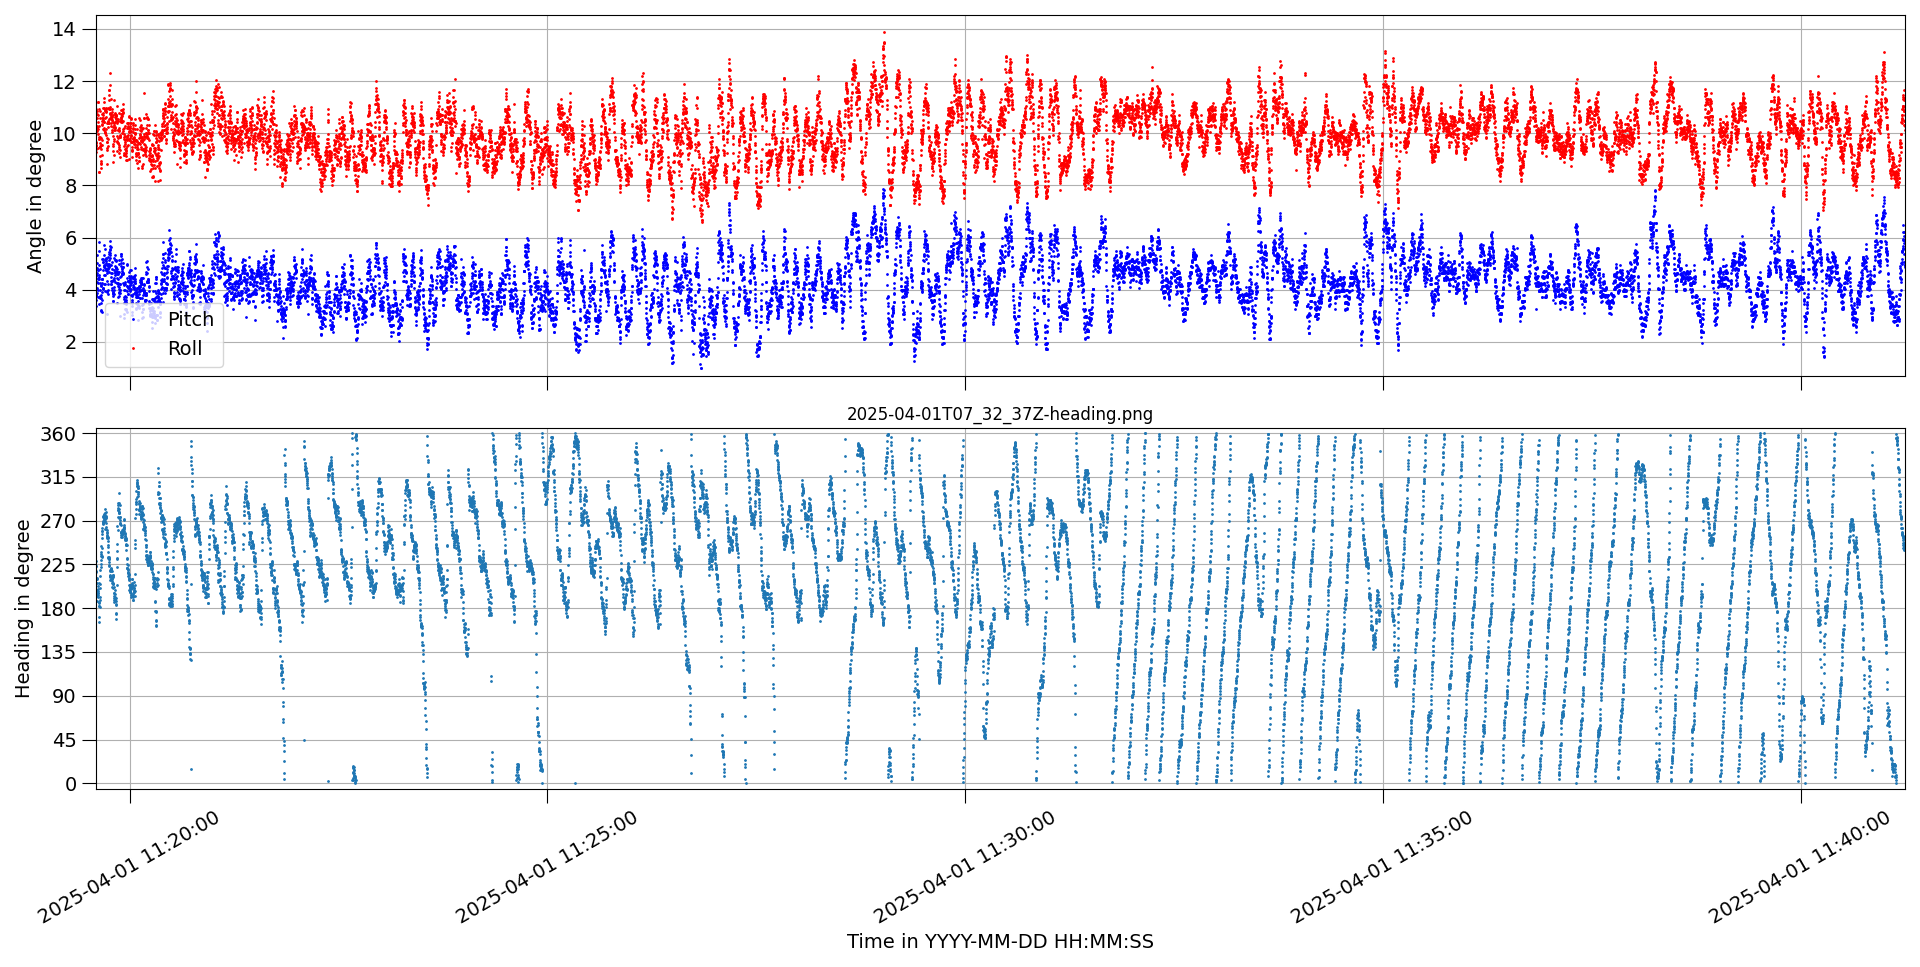
\includegraphics[width=\linewidth]{images/04_results/descend_heading.png}
    \caption[Heading during descent.]{Pitch, roll and heading during descent.}
    \label{fig:res:descent_heading}
\end{figure}